\documentclass[border=10pt]{standalone}
\usepackage[svgnames]{xcolor}
\usepackage{amsmath}
\usepackage{pgfplots}
\pgfplotsset{compat=newest}
\usepackage[sfdefault]{FiraSans}
\usepackage{FiraMono}
\renewcommand*\familydefault{\sfdefault}
\begin{document}
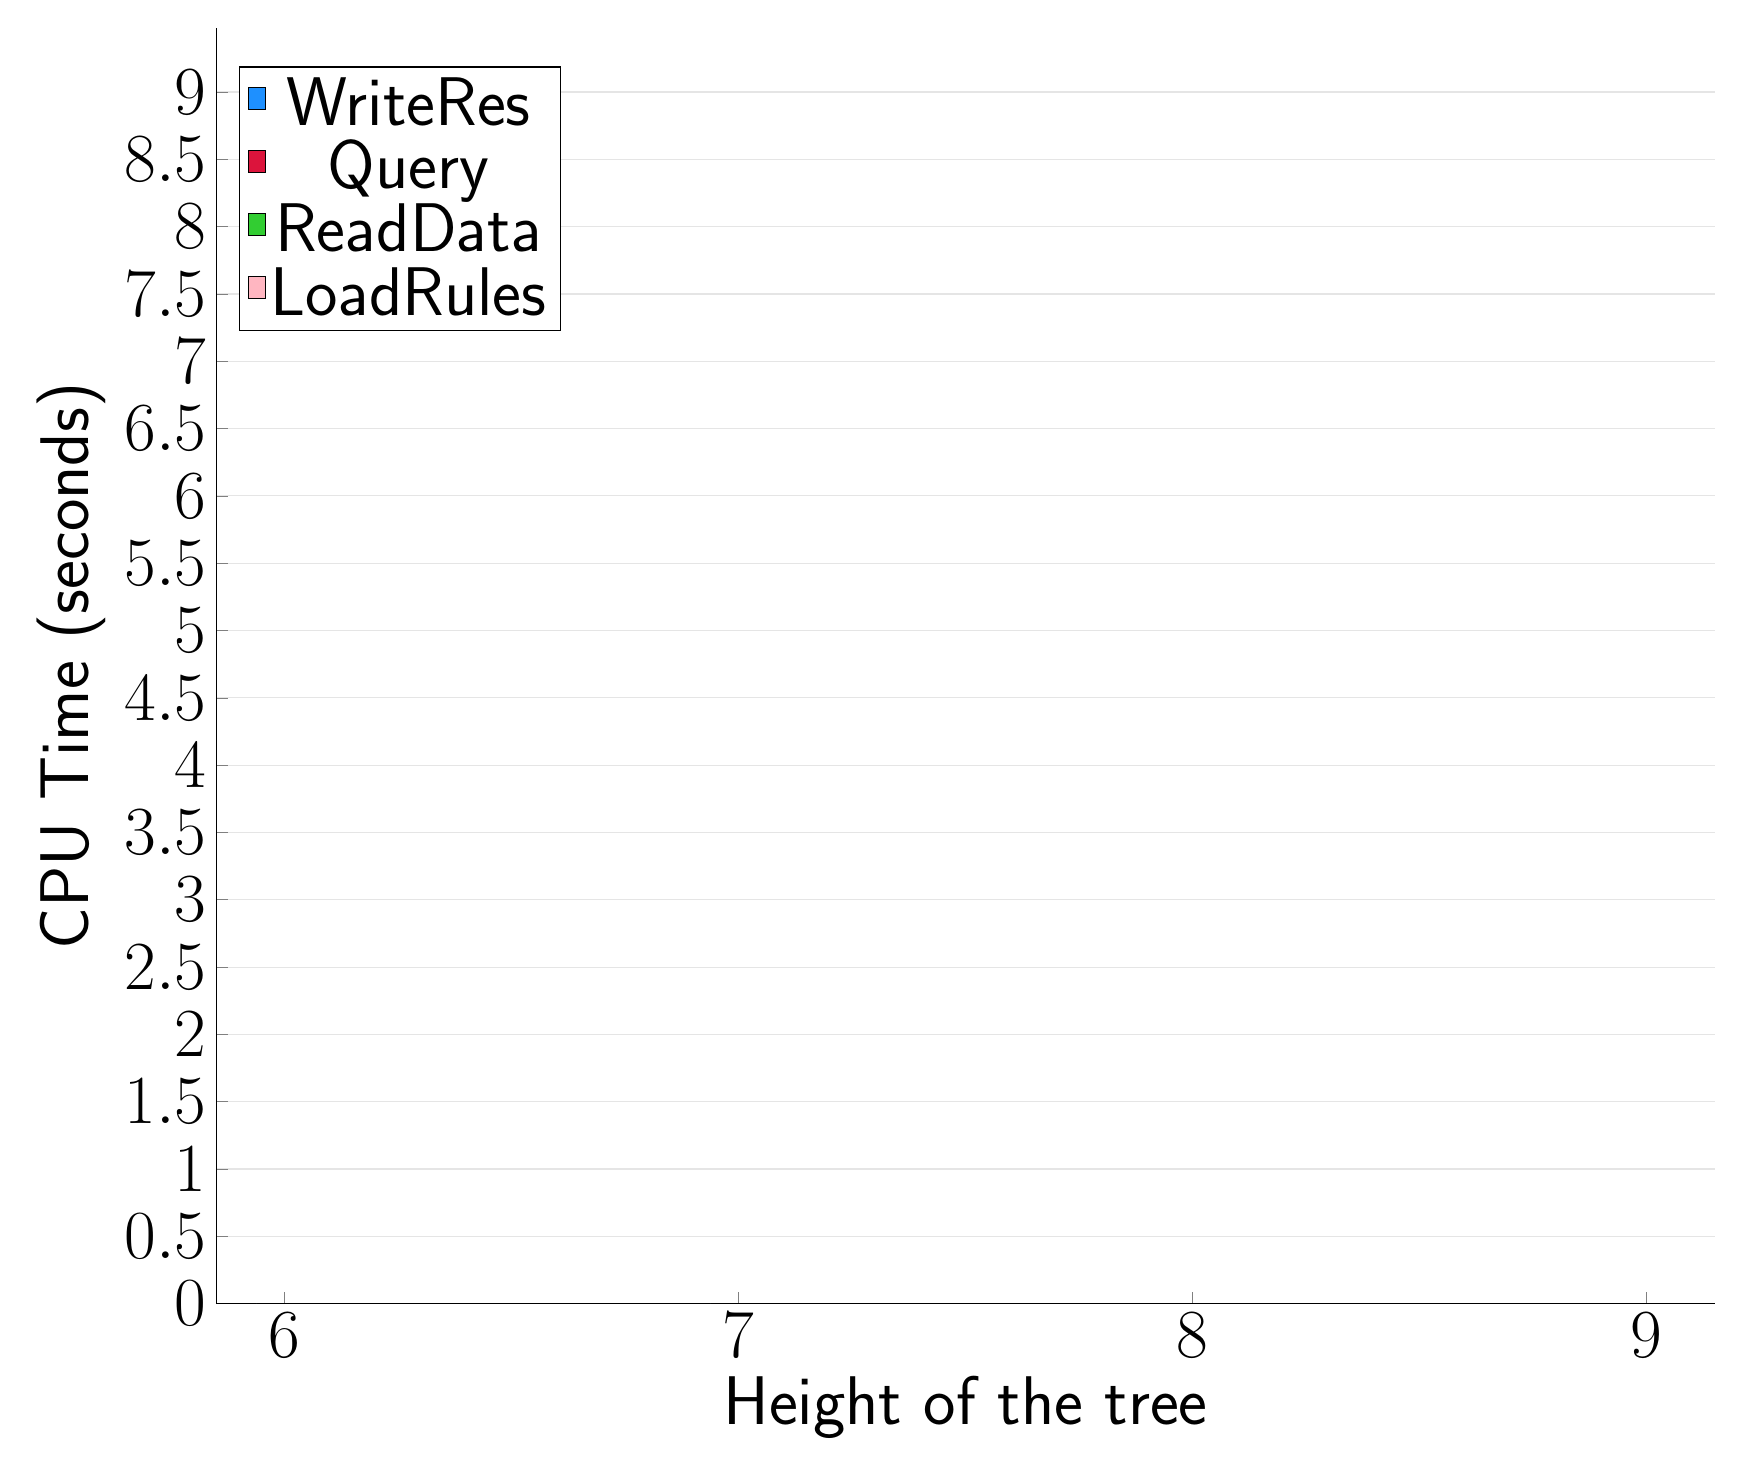
\begin{tikzpicture}
\begin{axis}[
   ybar stacked,
   width=1.7\textwidth,
   bar width=0.7cm,
   ymajorgrids, tick align=inside,
   major grid style={draw=gray!20},
   xtick=data,
   ymin=0, ymax=9.474,
   axis x line*=bottom,
   axis y line*=left,
   enlarge x limits=0.05,
   legend style={
       at={(0.23, 0.97)},
       anchor=north east,
       legend columns=1,
       font=\Huge,
   },
   ylabel={CPU Time (seconds)},
   xlabel={Height of the tree},
   label style={font=\Huge},
   tick label style={font=\Huge},
]
\addlegendimage{fill=DodgerBlue, draw=black, line width=0.2pt}
\addlegendentry{WriteRes}
\addlegendimage{fill=Crimson, draw=black, line width=0.2pt}
\addlegendentry{Query}
\addlegendimage{fill=LimeGreen, draw=black, line width=0.2pt}
\addlegendentry{ReadData}
\addlegendimage{fill=LightPink, draw=black, line width=0.2pt}
\addlegendentry{LoadRules}
\addplot +[fill=LightPink, draw=black, line width=0.2pt] coordinates {
(6, 0.0005501999999999998)
(7, 0.0005497999999999998)
(8, 0.0005487999999999996)
(8, 0.0005522000000000003)
(8, 0.0005491999999999996)
(9, 0.0005498000000000008)
(9, 0.0005568000000000002)
(9, 0.0005519999999999998)
(9, 0.0005482000000000004)
(9, 0.0005526000000000001)
};
\addplot +[fill=LimeGreen, draw=black, line width=0.2pt] coordinates {
(6, 0.0001718)
(7, 0.0002175999999999996)
(8, 0.00031600000000000063)
(8, 0.0003181999999999996)
(8, 0.00031560000000000003)
(9, 0.0005167999999999998)
(9, 0.0005247999999999999)
(9, 0.0005340000000000002)
(9, 0.0005198000000000002)
(9, 0.0005172000000000001)
};
\addplot +[fill=Crimson, draw=black, line width=0.2pt] coordinates {
(6, 3.200000000000008e-05)
(7, 6.180000000000005e-05)
(8, 0.0001307999999999996)
(8, 0.00013240000000000018)
(8, 0.0001301999999999998)
(9, 0.00029060000000000056)
(9, 0.00029160000000000026)
(9, 0.0002869999999999994)
(9, 0.0002923999999999994)
(9, 0.0002858000000000002)
};
\addplot +[fill=DodgerBlue, draw=black, line width=0.2pt] coordinates {
(6, 0.0002784000000000003)
(7, 0.0005976000000000004)
(8, 0.0013676000000000005)
(8, 0.0013715999999999997)
(8, 0.001373)
(9, 0.0030743999999999993)
(9, 0.0031005999999999994)
(9, 0.0031008000000000008)
(9, 0.0031228000000000007)
(9, 0.0030828)
};
\end{axis}
\end{tikzpicture}

\end{document}
